\documentclass[11pt,a4paper]{article}
\usepackage[utf8]{inputenc}
\usepackage[T1]{fontenc}
\usepackage[italian]{babel}
\usepackage[margin=2.5cm]{geometry}
\usepackage{amsmath,amssymb,amsthm}
\usepackage{graphicx}
\usepackage{booktabs}
\usepackage{xcolor}
\usepackage[hidelinks]{hyperref}
\usepackage{tcolorbox}

\newcommand{\scal}[2]{\left\langle #1,\, #2 \right\rangle}
\newcommand{\norm}[1]{\left\lVert #1 \right\rVert}
\newcommand{\e}{\mathrm{e}}
\newcommand{\dt}{\Delta t}
\newtcolorbox{idea}{colback=blue!4,colframe=blue!40,boxrule=0.5pt,arc=2pt,left=6pt,right=6pt,top=4pt,bottom=4pt}
\newtheorem*{lemma}{Lemma di Neyman--Pearson}

\title{Uno stimatore di verosimiglianza per il pile-up\\[2pt]
\large derivazione passo per passo}
\author{Note per la tesi -- misura m205, rivelatori di luce CUPID}
\date{23 settembre 2026}

\begin{document}
\maketitle

\begin{idea}
\textbf{In una frase.} Per ogni evento lo stimatore $M$ risponde alla domanda:
\emph{``è più verosimile che questo evento sia un pile-up di due impulsi --- con un ritardo e una
ripartizione d'energia qualsiasi, pesati con quanto sono probabili --- oppure un impulso singolo?''}
Si rigettano gli eventi per cui la risposta pende abbastanza verso il pile-up.
\end{idea}

\noindent Il percorso:
\begin{enumerate}
  \item si scrive come è fatto un evento (singolo o pile-up) e come è fatto il rumore;
  \item si definisce una ``distanza'' fra un evento e un modello, pesata con il rumore;
  \item si impara ad adattare un template con ampiezza e tempo ignoti: è il filtro ottimo;
  \item si scrive il template del pile-up e si scopre che basta la correlazione del filtro ottimo;
  \item si confronta pile-up e singolo per un ritardo fissato;
  \item si passa a tutti i ritardi: il lemma di Neyman--Pearson dice come combinarli per minimizzare il BI.
\end{enumerate}
Nelle sezioni~\ref{sec:limiti} e~\ref{sec:risultati} si vede cosa fa lo stimatore e quanto guadagna;
nella sezione~\ref{sec:fonti} si dice da dove viene ogni passaggio.

%==========================================================================================
\section{Il modello dei dati}
%==========================================================================================
Si lavora in frequenza. Le quantità:

\begin{center}
\begin{tabular}{ll}
\toprule
$X_k$ & trasformata di Fourier dell'evento, alla frequenza angolare $\omega_k$ \\
$S_k$ & trasformata del template (impulso medio, picco $=1$)\footnotemark \\
$J_k$ & densità spettrale del rumore (NPS) \\
$A,\ t_0$ & ampiezza totale e tempo di arrivo, \emph{ignoti} \\
$\dt,\ r$ & ritardo fra i due impulsi e frazione d'energia del secondo \\
\bottomrule
\end{tabular}
\end{center}
\footnotetext{Come nel resto del codice, $S$ è la trasformata del template moltiplicato per una
finestra di Hann (\texttt{compute\_H}).}

\paragraph{Impulso singolo.} Un impulso di ampiezza $A$ che arriva al tempo $t_0$ è
\begin{equation}
  X_k = A\, S_k\, \e^{-i\omega_k t_0} + N_k .
\end{equation}
Il fattore $\e^{-i\omega t_0}$ è il teorema di traslazione di Fourier: un ritardo nel tempo è una
fase in frequenza.

\paragraph{Pile-up.} Due impulsi con la \emph{stessa forma}: il primo porta la frazione $1-r$
dell'energia e arriva a $t_0$, il secondo porta $r$ e arriva $\dt$ dopo:
\begin{equation}
  X_k = A\, S_k\, \e^{-i\omega_k t_0}\,\Big[(1-r) + r\, \e^{-i\omega_k \dt}\Big] + N_k .
  \label{eq:pileup}
\end{equation}
Chiamo $\theta = (\dt, r)$ i due parametri che distinguono un pile-up dall'altro.

\paragraph{Rumore.} Gaussiano e stazionario. La stazionarietà rende indipendenti le diverse
frequenze, ciascuna con varianza proporzionale a $J_k$. Sono esattamente le ipotesi del filtro
ottimo: non se ne aggiungono altre.

%==========================================================================================
\section{Una distanza pesata con il rumore}
%==========================================================================================
\begin{idea}
L'idea: confrontare l'evento con un modello frequenza per frequenza, ma dando \emph{meno peso alle
frequenze più rumorose}, perché lì una differenza significa poco.
\end{idea}
Il prodotto scalare e la norma che lo realizzano sono
\begin{equation}
  \scal{a}{b} = \sum_k \frac{\mathrm{Re}\!\left(a_k\, b_k^{*}\right)}{J_k},
  \qquad \norm{a}^2 = \scal{a}{a},
  \label{eq:metrica}
\end{equation}
con la somma su tutte le frequenze. È il prodotto scalare ordinario con ogni termine diviso per il
rumore di quella frequenza.

Con la normalizzazione della NPS usata nel codice, la proiezione del rumore su una direzione $u$
ha varianza
\begin{equation}
  \mathrm{Var}\,\scal{N}{u} = \norm{u}^2 .
  \label{eq:varianza}
\end{equation}
È la stessa convenzione per cui la risoluzione del filtro ottimo vale
$\sigma_\mathrm{OF} = 1/\sqrt{\sum_k |S_k|^2/J_k}$; è verificata sul Monte Carlo
($\sigma_\text{simulata}/\sigma_\mathrm{OF} = 0.99$).

Per un rumore gaussiano con questa proprietà, la probabilità di osservare $X$ se il modello
(senza rumore) è $m$ vale
\begin{equation}
  \ln p(X \mid m) = -\tfrac12 \norm{X - m}^2 + \text{costante}.
  \label{eq:verosimiglianza}
\end{equation}
In parole: \emph{un modello è tanto più verosimile quanto più è vicino all'evento, misurando la
distanza in unità di rumore.} Di conseguenza, per due modelli $m_1$ e $m_2$,
\begin{equation}
  \ln \frac{p(X\mid m_1)}{p(X\mid m_2)} = \tfrac12\Big(\norm{X-m_2}^2 - \norm{X-m_1}^2\Big):
  \label{eq:rapporto}
\end{equation}
il logaritmo del rapporto di verosimiglianza è metà del $\chi^2$ che $m_1$ lascia \emph{in meno}
rispetto a $m_2$.

%==========================================================================================
\section{Adattare un template con ampiezza e tempo ignoti}
\label{sec:fit}
%==========================================================================================
Prendiamo un template qualsiasi $T$, spostato al tempo $t$ e moltiplicato per un'ampiezza $a\geq0$.
Sviluppando il quadrato,
\begin{equation}
  \norm{X - a\, T \e^{-i\omega t}}^2
  = \norm{X}^2 - 2a\, c_T(t) + a^2 \norm{T}^2,
  \qquad c_T(t) = \scal{X}{T\,\e^{-i\omega t}},
\end{equation}
dove si è usato $\norm{T\e^{-i\omega t}} = \norm{T}$ (una fase non cambia il modulo).

Per $t$ fissato è una parabola in $a$. Il minimo sta in $\hat a = \max(0, c_T)/\norm{T}^2$ (il
vincolo $a\geq0$ vieta ampiezze negative), e lì il $\chi^2$ scende di
$\max(0,c_T)^2/\norm{T}^2$. Scegliendo anche il tempo migliore:
\begin{equation}
  \boxed{\;L_T = \max_t\, \frac{\max\!\big(0,\ c_T(t)\big)^2}{\norm{T}^2}\;}
  \label{eq:LT}
\end{equation}
$L_T$ è \textbf{il $\chi^2$ spiegato dal template}: quanta parte dell'evento, in unità di rumore al
quadrato, il template riesce a rendere conto. Sostituire le grandezze ignote ($a$, $t$) con il loro
valore migliore si chiama \emph{profilare} la verosimiglianza.

\paragraph{Il caso dell'impulso singolo è il filtro ottimo.} Con $T = S$:
\begin{equation}
  y(t) \equiv c_S(t) = \sum_k \frac{X_k\, S_k^{*}\, \e^{i\omega_k t}}{J_k},
  \qquad
  L_1 = \max_t \frac{y(t)^2}{R(0)},
  \qquad R(0) = \norm{S}^2 = \sum_k \frac{|S_k|^2}{J_k}.
  \label{eq:y}
\end{equation}
$y(t)$ è la \emph{correlazione del filtro ottimo}: si calcola con una sola FFT inversa, ed è la
stessa quantità che l'OF massimizza per trovare ampiezza e tempo. Infatti
$\hat A = y(\hat t)/R(0)$ è l'ampiezza dell'OF, e
\begin{equation}
  L_1 = \left(\frac{\hat A}{\sigma_\mathrm{OF}}\right)^2
\end{equation}
è il quadrato del rapporto segnale/rumore dell'evento visto dal filtro ottimo.

%==========================================================================================
\section{Il template del pile-up}
%==========================================================================================
Per un pile-up con $\theta=(\dt,r)$ fissato, il template è dato dalla~\eqref{eq:pileup}:
\begin{equation}
  P_\theta = S\,\Big[(1-r) + r\,\e^{-i\omega\dt}\Big].
\end{equation}
Servono le due quantità della~\eqref{eq:LT}. La prima si ottiene dalla linearità del prodotto
scalare e dal teorema di traslazione:
\begin{align}
  c_{P_\theta}(t)
  &= (1-r)\scal{X}{S\e^{-i\omega t}} + r\,\scal{X}{S\e^{-i\omega(t+\dt)}} \nonumber\\
  &= (1-r)\, y(t) + r\, y(t+\dt).
  \label{eq:cP}
\end{align}
La seconda, usando $\big|(1-r)+r\e^{-i\omega\dt}\big|^2 = (1-r)^2 + r^2 + 2r(1-r)\cos(\omega\dt)$:
\begin{equation}
  \norm{P_\theta}^2 = \big[(1-r)^2 + r^2\big] R(0) + 2r(1-r)\, R(\dt),
  \qquad
  R(\tau) = \sum_k \frac{|S_k|^2 \cos(\omega_k\tau)}{J_k}.
  \label{eq:normP}
\end{equation}
$R(\tau)$ è l'\emph{autocorrelazione del template} nella metrica del rumore: quanto il template
somiglia a se stesso spostato di $\tau$. Mettendo insieme:
\begin{equation}
  \boxed{\;L(\theta) = \max_t \frac{\max\!\big(0,\ (1-r)\,y(t) + r\,y(t+\dt)\big)^2}
  {\big[(1-r)^2 + r^2\big] R(0) + 2r(1-r)\, R(\dt)}\;}
  \label{eq:Ltheta}
\end{equation}

\begin{idea}
\textbf{Perché il metodo è praticabile.} Tutto dipende dall'evento solo attraverso $y(t)$, la
correlazione che l'OF calcola già. $R(\tau)$ dipende solo dal template e dalla NPS: si calcola una
volta per canale e punto di lavoro. Provare centinaia di pile-up diversi non costa nessuna FFT in
più: servono solo combinazioni di $y$ letta a due tempi.
\end{idea}

%==========================================================================================
\section{Pile-up contro singolo, per un pile-up fissato}
%==========================================================================================
Dalla~\eqref{eq:rapporto}, usando per ciascuna ipotesi il suo adattamento migliore:
\begin{equation}
  \ln \frac{\max_{A,t_0} p(X\mid \text{pile-up } \theta)}{\max_{A,t_0} p(X\mid \text{singolo})}
  = \tfrac12\Big[L(\theta) - L_1\Big].
  \label{eq:LRtheta}
\end{equation}
In parole: \emph{di quanto il miglior pile-up con questi $\dt$ e $r$ spiega l'evento meglio del
miglior impulso singolo.} Per $\dt = 0$ il template del pile-up coincide con quello singolo e la
differenza è zero.

Se si conoscesse in anticipo $\theta$, questa sarebbe la statistica da usare. Ma $\theta$ cambia da
un pile-up all'altro: serve un modo di combinare tutti i $\theta$.

%==========================================================================================
\section{Da un pile-up fissato a tutti: perché la media}
\label{sec:media}
%==========================================================================================

\subsection{Il lemma di Neyman--Pearson}
\begin{lemma}
Per decidere fra due ipotesi \emph{semplici} (completamente specificate) $H_0$ e $H_1$, fra tutti i
test che rigettano $H_0$ con la stessa probabilità $\alpha$ quando $H_0$ è vera, il più potente ---
quello che, quando è vera $H_1$, rigetta $H_0$ il più spesso possibile --- è: rigettare $H_0$ quando
\begin{equation}
  \frac{p(X\mid H_1)}{p(X\mid H_0)} > k,
\end{equation}
con la soglia $k$ scelta in modo da ottenere proprio la probabilità $\alpha$~\cite{NP1933}.
\end{lemma}
\noindent Nel nostro caso $H_0$ = ``impulso singolo'', $\alpha = 0.1$ (si accetta il 90\% dei
singoli), e ``rigettare $H_0$'' significa riconoscere l'evento come pile-up. Una dimostrazione breve
è in appendice~\ref{app:NP}.

\subsection{Il BI è una media sui pile-up}
Il BI conta i pile-up che sopravvivono al taglio, \emph{mediati} su come si presentano:
\begin{equation}
  \mathrm{BI} = K \int \pi(\theta)\; P\big(\text{sopravvive}\mid\theta\big)\, d\theta
  = K\Big[1 - \int \pi(\theta)\; P\big(\text{rigettato}\mid\theta\big)\, d\theta\Big],
\end{equation}
dove $\pi(\theta)$ è la distribuzione vera dei pile-up (sezione~\ref{sec:prior}). Ora il passaggio
chiave. Se $\mathcal{R}$ è l'insieme degli eventi rigettati,
\begin{equation}
  \int \pi(\theta)\, P(\text{rigettato}\mid\theta)\, d\theta
  = \int \pi(\theta) \int_{\mathcal{R}} p(X\mid\theta)\, dX\, d\theta
  = \int_{\mathcal{R}} \underbrace{\int \pi(\theta)\, p(X\mid\theta)\, d\theta}_{\bar p_1(X)}\; dX ,
\end{equation}
dove si sono solo scambiati gli integrali. La potenza \emph{media} contro tutti i pile-up è quindi
la potenza contro \textbf{un'unica ipotesi semplice}: ``$X$ è stato generato dalla miscela
$\bar p_1$'', cioè da un pile-up con $\theta$ estratto da $\pi$. Il lemma allora dice che, a
accettanza dei singoli fissata, il test che minimizza il BI è
\begin{equation}
  \Lambda(X) = \frac{\bar p_1(X)}{p_0(X)} = \int \pi(\theta)\, \frac{p(X\mid\theta)}{p_0(X)}\, d\theta .
  \label{eq:Lambda}
\end{equation}
Questo passaggio è esatto: minimizzare il BI \emph{è} un problema di Neyman--Pearson contro la
miscela. È il criterio della \emph{potenza media pesata} della letteratura
statistica~\cite{Wald1943,AndrewsPloberger1994}.

\subsection{Ampiezza e tempo ignoti: la statistica $M$}
In entrambe le ipotesi ampiezza e tempo sono ignoti, quindi nessuna delle due è davvero semplice.
Si fa la scelta standard: si sostituisce ogni verosimiglianza con il suo massimo su $A$ e
$t_0$ (verosimiglianza profilata~\cite{CCGV2011}). Con la~\eqref{eq:LRtheta}, e scrivendo
l'integrale come somma su una griglia di valori di $\theta$ con pesi $\pi(\theta)$ normalizzati,
\begin{equation}
  \boxed{\; M = \ln \sum_{\theta} \pi(\theta)\; \exp\!\Big[\tfrac12\big(L(\theta) - L_1\big)\Big] \;}
  \label{eq:M}
\end{equation}
Profilare invece di integrare su ampiezza e tempo è un'approssimazione: per questo $M$ è
\emph{vicino} al test ottimo, non esattamente il test ottimo.

\paragraph{Perché la media e non il massimo.} Il test di verosimiglianza più comune (GLRT) prende il
\emph{massimo} su $\theta$ invece della media. Risponde a un'altra domanda --- quanto somiglia
l'evento al pile-up che gli somiglia di più --- e non minimizza il BI. Misurato: da solo è peggio
del rapporto dei massimi del 9\% su ch31, mentre $M$ è meglio del 2\%.

\subsection{La distribuzione dei pile-up}
\label{sec:prior}
$\pi(\dt, r) = \pi(\dt)\,\pi(r)$:
\begin{itemize}
  \item $\dt$ \textbf{uniforme} fra 0 e $\dt_\text{max} = 0.8$~ms: le coincidenze casuali sono
    poissoniane, quindi il secondo evento cade con la stessa probabilità in qualsiasi punto della
    finestra. $\dt_\text{max}$ è lo stesso usato dal BI analitico e dal Monte Carlo.
  \item $r$ secondo la distribuzione della ripartizione d'energia fra i due eventi
    (\texttt{pdf\_ratio2b}), la stessa del BI analitico e del Monte Carlo~\cite{Chernyak2012}.
\end{itemize}
Se $\pi$ fosse sbagliata il test resterebbe valido (l'accettanza dei singoli si fissa comunque al
90\%), ma non sarebbe più ottimo.

%==========================================================================================
\section{Il taglio e il BI}
%==========================================================================================
La distribuzione di $M$ sui singoli non ha una forma chiusa. Si procede esattamente come per il
rapporto dei massimi: si calcola $M$ su impulsi singoli simulati, si prende la soglia $c$ che ne
lascia passare il 90\%, si rigettano gli eventi con $M > c$, e
\begin{equation}
  \mathrm{BI} = K \times \text{(frazione di pile-up simulati con } M \leq c).
\end{equation}
Non c'è niente da addestrare: servono solo il template, la NPS e la soglia.

%==========================================================================================
\section{Cosa fa $M$: i due regimi}
\label{sec:limiti}
%==========================================================================================

\subsection{Ritardo piccolo: $M$ misura la larghezza dell'impulso}
Si sviluppa la~\eqref{eq:cP} attorno al \emph{baricentro temporale} $u = t + r\dt$ dei due impulsi:
\begin{equation}
  (1-r)\,y(u - r\dt) + r\,y\big(u + (1-r)\dt\big)
  = y(u) + \underbrace{\big[-(1-r)r + r(1-r)\big]}_{=\,0}\dt\; y'(u) + \tfrac12\, \varepsilon\, y''(u)
  + O(\dt^3),
\end{equation}
con
\begin{equation}
  \varepsilon = r(1-r)\,\dt^2 ,
\end{equation}
la varianza della distribuzione dei tempi dei due impulsi. Il termine al prim'ordine si cancella:
\textbf{un pile-up molto stretto è, al prim'ordine, solo un impulso spostato}, indistinguibile da un
singolo arrivato un po' dopo. Il primo effetto osservabile è un \emph{allargamento} simmetrico, di
entità $\varepsilon$. Nella~\eqref{eq:normP}, con
$R(\dt) = R(0) - \tfrac12 M_2 \dt^2 + O(\dt^4)$ e $M_n = \sum_k \omega_k^n |S_k|^2/J_k$
(quindi $M_0 = R(0)$):
\begin{equation}
  \norm{P_\theta}^2 = M_0 - \varepsilon\, M_2 + O(\dt^4).
\end{equation}
Derivando $L = c_P^2/\norm{P}^2$ rispetto a $\varepsilon$ in $\varepsilon = 0$:
\begin{equation}
  L(\theta) - L_1 = \varepsilon\;\frac{y}{M_0}\,\Big[y'' + \frac{M_2}{M_0}\, y\Big] + O(\varepsilon^2)
  = \varepsilon\; \hat A\; \scal{X}{g\,\e^{-i\omega \hat t}} + O(\varepsilon^2),
  \label{eq:piccolo}
\end{equation}
dove $\hat A = y/M_0$ è l'ampiezza dell'OF e
\begin{equation}
  g = S\left(\frac{M_2}{M_0} - \omega^2\right).
\end{equation}
Si è usato $y''(t) = \scal{X}{-\omega^2 S\,\e^{-i\omega t}}$. Il fattore $(M_2/M_0 - \omega^2)$ è
positivo sotto la frequenza $f_0 = \sqrt{M_2/M_0}/2\pi$ e negativo sopra: $g$ misura
\emph{contenuto a bassa frequenza meno contenuto ad alta frequenza}, bilanciato in modo che su un impulso singolo dia esattamente zero
($\scal{S}{g} = 0$). Un pile-up ha le alte frequenze smorzate e dà un valore positivo. Normalizzato,
$T = \scal{X}{g\,\e^{-i\omega\hat t}}/\norm{g}$ è lo \textbf{stimatore di larghezza}, con media 0 e
varianza 1 sui singoli.

Il termine al prim'ordine in $\varepsilon$ è la derivata della log-verosimiglianza rispetto
all'allargamento: il test che usa solo questo termine è il \emph{test del punteggio}, il più potente
contro allargamenti piccoli (localmente più potente)~\cite{CoxHinkley1974}. Quindi, a piccoli
$\dt$, $M$ si comporta come lo stimatore di larghezza, e questo coincide in pratica con quello che
fanno i filtri di banda addestrati (correlazione 0.95--0.99 sui singoli). Tutti e tre lì stanno sul
limite teorico: è la regione da cui viene il 78\% del BI su ch31 (figura~\ref{fig:sopravvivenza}b),
e \emph{nessuno stimatore può fare meglio}.

\subsection{Ritardo grande: $M$ cerca un secondo impulso}
Quando i due impulsi sono ben separati, $R(\dt)\approx 0$ (i due template spostati non si
sovrappongono nella metrica del rumore). Senza rumore,
$y(t_0) \approx (1-r)\,A\,R(0)$ e $y(t_0+\dt) \approx r\,A\,R(0)$, quindi
\begin{align}
  L(\theta) &\approx A^2 R(0)\, \big[(1-r)^2 + r^2\big], \nonumber\\
  L_1 &\approx A^2 R(0)\, \max(r, 1-r)^2 \quad\text{(il singolo si adatta all'impulso maggiore)}, \nonumber\\
  L(\theta) - L_1 &\approx A^2 R(0)\, \min(r, 1-r)^2
  = \Big(\mathrm{SNR}\cdot \min(r,1-r)\Big)^2 .
  \label{eq:grande}
\end{align}
\textbf{Riconoscere un pile-up ben separato equivale a rivelare l'impulso più piccolo da solo}, con
tutto il suo rapporto segnale/rumore; e questo migliora al crescere della separazione. Il rapporto
dei massimi invece \emph{satura}: quando gli impulsi si separano, il massimo della banda alta si
aggancia all'impulso maggiore e il rapporto smette di dipendere da $\dt$. È esattamente dove $M$
guadagna (figura~\ref{fig:sopravvivenza}a).

\begin{figure}[t]
  \centering
  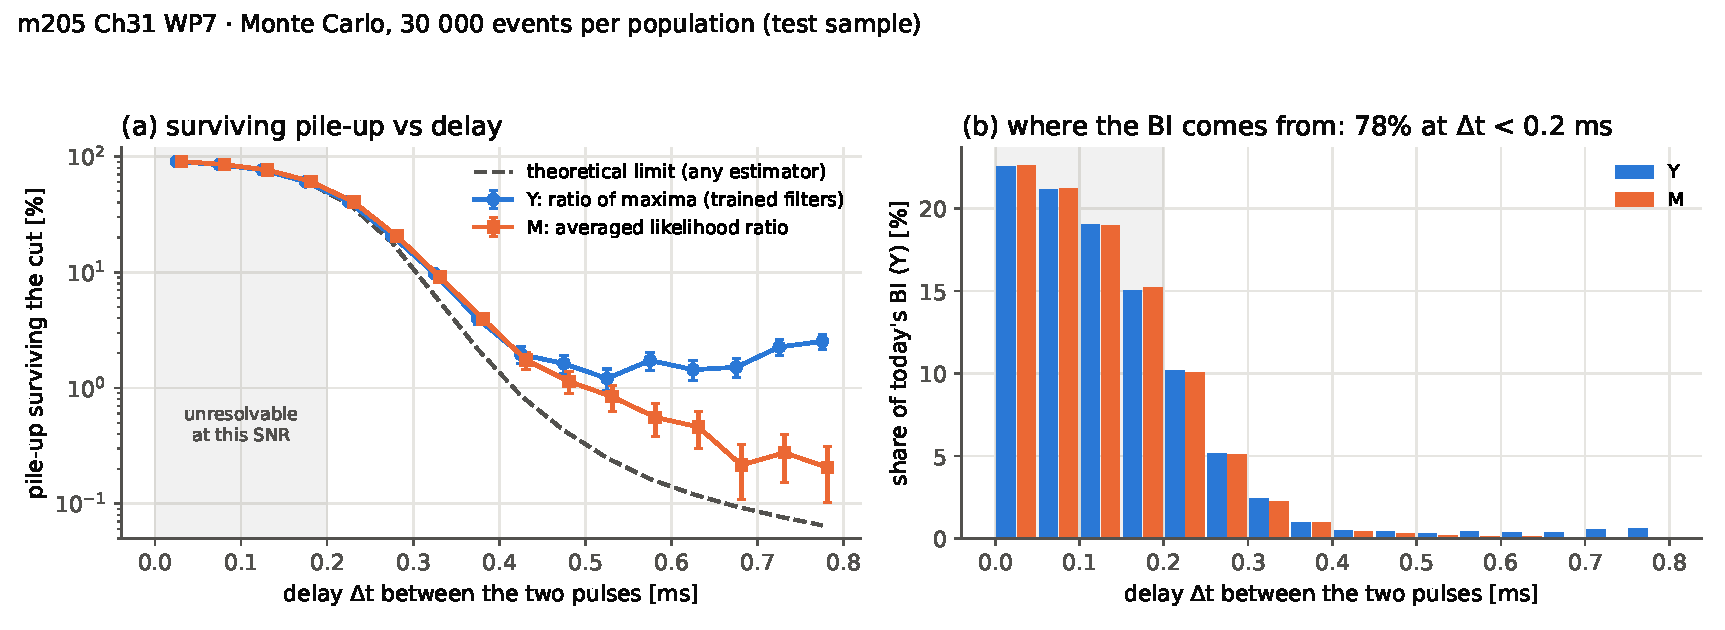
\includegraphics[width=\textwidth]{fig_M_survival_ch31_wp7.pdf}
  \caption{Ch31 WP7, Monte Carlo, 30\,000 eventi per popolazione. (a)~Frazione di pile-up che
  sopravvive al taglio in funzione del ritardo: rapporto dei massimi ($Y$), stimatore $M$ e limite
  teorico. Oltre $\sim$0.45~ms $Y$ smette di migliorare, $M$ continua a scendere. (b)~Da dove viene
  il BI: il 78\% da pile-up con $\dt<0.2$~ms, dove $Y$, $M$ e il limite coincidono.}
  \label{fig:sopravvivenza}
\end{figure}

%==========================================================================================
\section{Implementazione}
%==========================================================================================
\begin{itemize}
  \item $y(t)$ si calcola su una griglia fine (passo 0.01~ms), perché il campionamento (0.1~ms) è
    troppo grosso rispetto ai ritardi in gioco: somma diretta sulle frequenze che portano il
    99.9999\% del peso $|S|^2/J$.
  \item $t$ entro $\pm0.5$~ms dalla posizione nominale; $\dt$ da 0 a 0.8~ms (81 valori);
    $r$ da 0.05 a 0.95 (19 valori).
  \item La somma della~\eqref{eq:M} si calcola in forma logaritmica (\texttt{logsumexp}): per pile-up
    evidenti $L(\theta)-L_1$ arriva a centinaia e l'esponenziale andrebbe fuori scala.
  \item Nella verosimiglianza il template è l'AP simulato, lo stesso su cui sono addestrati i filtri
    di banda; gli eventi del Monte Carlo sono generati dal fit.
  \item Costo: circa 6~ms per evento. Codice: \texttt{test/likelihood\_estimator\_m205.py}.
\end{itemize}

%==========================================================================================
\section{Risultati}
\label{sec:risultati}
%==========================================================================================
Riferimento: il rapporto dei massimi $Y$ con i filtri Wiener addestrati (campagna \texttt{\_swna1\_hist}).
Per ciascuno stimatore il taglio accetta il 90\% dei singoli; le differenze sono misurate sugli
\emph{stessi eventi}, con errore da bootstrap appaiato.

\begin{center}
\begin{tabular}{lrccc}
\toprule
punto & SNR$_\mathrm{OF}$ & $M$ vs $Y$ & $M$ vs $Y$ & limite teorico \\
      &                   & campione indipendente & eventi della campagna & vs $Y$ \\
\midrule
Ch31 WP7  &  20 & $-2.32 \pm 0.42\%$ & $-1.96 \pm 0.32\%$ & $-5.6\%$ \\
Ch91 WP15 &  25 & $-1.75 \pm 0.27\%$ & $-1.51 \pm 0.23\%$ & $-5.1\%$ \\
Ch34 WP15 & 124 & $-0.41 \pm 0.31\%$ & $-0.31 \pm 0.23\%$ & $-2.4\%$ \\
\bottomrule
\end{tabular}
\end{center}

\begin{itemize}
  \item \textbf{Campione indipendente}: 30\,000 eventi per popolazione, semi diversi da quelli della
    campagna. \textbf{Eventi della campagna}: il Monte Carlo ufficiale (seme 1234, 50\,000 eventi),
    rigenerato; $Y$ ne riproduce il BI a tutte le cifre, quindi sono gli stessi eventi.
  \item Il guadagno è $\sim$2\% dove l'SNR è basso e non misurabile dove è alto, dove $Y$ è già a meno
    del 2.4\% dal limite.
  \item Usando nella verosimiglianza il template \emph{vero} (il fit che genera gli eventi) invece
    dell'AP simulato, il risultato non cambia ($-2.24$, $-1.72$, $-0.48\%$): il guadagno non viene
    dal conoscere la verità.
  \item \textbf{Il limite teorico} è, per ogni $\theta$, la distanza del pile-up dagli impulsi
    singoli $d(\theta) = \min_{a,t}\norm{A P_\theta - a S\e^{-i\omega t}}$, con sopravvivenza
    $\Phi(z_{0.9} - d)$. È calcolato come se si conoscesse $\theta$ in anticipo: nessun test singolo
    lo raggiunge, e il vero ottimo raggiungibile sta fra $M$ e il limite.
\end{itemize}

%==========================================================================================
\section{Ipotesi e limiti}
%==========================================================================================
\begin{itemize}
  \item Rumore gaussiano e stazionario descritto dalla NPS: le stesse ipotesi del filtro ottimo.
  \item Forma dell'impulso nota e uguale per i due impulsi del pile-up.
  \item Ampiezza e tempo sono profilati, non integrati: $M$ è un'approssimazione del test ottimo.
  \item La soglia si fissa su impulsi singoli simulati; sui dati reali andrebbe calibrata su un
    campione di singoli, come per $Y$.
  \item I risultati sono su tre punti di lavoro: per un numero da tesi va ripetuto su tutti i canali
    e punti di lavoro con il Monte Carlo a 50 semi.
\end{itemize}

%==========================================================================================
\section{Da dove viene ogni passaggio}
\label{sec:fonti}
%==========================================================================================
\begin{center}
\begin{tabular}{p{0.46\textwidth}p{0.46\textwidth}}
\toprule
passaggio & fonte \\
\midrule
Verosimiglianza gaussiana in frequenza, filtro ottimo, $\sigma_\mathrm{OF}$
  & standard~\cite{GattiManfredi1986,Kay1998,Alduino2016} \\
Adattamento di un template con ampiezza e tempo ignoti (sez.~\ref{sec:fit})
  & standard (\emph{matched filter})~\cite{Kay1998,VanTrees1968} \\
Lemma di Neyman--Pearson & \cite{NP1933} \\
Potenza media su $\pi(\theta)$ = potenza contro la miscela; statistica esponenziale-mediata
  & \emph{weighted average power}~\cite{Wald1943,AndrewsPloberger1994}; test di ipotesi composite
  con parametri casuali~\cite{VanTrees1968,Kay1998} \\
Verosimiglianza profilata & \cite{CCGV2011} \\
Test del punteggio / localmente più potente & \cite{CoxHinkley1974} \\
Distribuzione della ripartizione d'energia nei pile-up di eventi $2\nu\beta\beta$ & \cite{Chernyak2012} \\
\midrule
Riduzione del template di pile-up a $y(t)$ e $R(\tau)$ [eq.~\eqref{eq:cP}--\eqref{eq:Ltheta}];
  identificazione del BI con la potenza media; limiti a piccolo e grande $\dt$ applicati al pile-up
  & \textbf{derivati in questo lavoro}, a partire dai risultati standard sopra \\
\bottomrule
\end{tabular}
\end{center}
Non è noto a chi scrive un lavoro che applichi esattamente questo stimatore al pile-up nei
rivelatori bolometrici, ma non è stato verificato in modo sistematico: prima di presentarlo come
nuovo va controllata la letteratura.

%==========================================================================================
\appendix
\section{Dimostrazione breve del lemma di Neyman--Pearson}
\label{app:NP}
%==========================================================================================
Sia $\phi^*(X)=1$ se $p_1(X)/p_0(X)>k$ e $0$ altrimenti (il test del lemma), e $\phi$ un qualsiasi
altro test con la stessa probabilità di rigettare $H_0$ quando è vera,
$\int\phi\,p_0 = \int\phi^*p_0 = \alpha$. Per costruzione $(\phi^*-\phi)(p_1 - k p_0) \geq 0$ per
ogni $X$: dove $p_1 > k p_0$ vale $\phi^* = 1 \geq \phi$, altrove $\phi^* = 0 \leq \phi$.
Integrando:
\begin{equation*}
  \int(\phi^*-\phi)\,p_1 \;\geq\; k \int(\phi^*-\phi)\,p_0 = 0 .
\end{equation*}
Quindi $\int\phi^* p_1 \geq \int \phi\, p_1$: nessun test con lo stesso $\alpha$ rigetta più
spesso $H_0$ quando è vera $H_1$.

%==========================================================================================
\begin{thebibliography}{99}
\bibitem{NP1933} J.~Neyman, E.~S.~Pearson, \emph{On the problem of the most efficient tests of
  statistical hypotheses}, Phil.\ Trans.\ R.\ Soc.\ A \textbf{231} (1933) 289--337.
\bibitem{GattiManfredi1986} E.~Gatti, P.~F.~Manfredi, \emph{Processing the signals from solid-state
  detectors in elementary-particle physics}, Riv.\ Nuovo Cimento \textbf{9} (1986) 1--146.
\bibitem{Kay1998} S.~M.~Kay, \emph{Fundamentals of Statistical Signal Processing, Vol.~II: Detection
  Theory}, Prentice Hall (1998).
\bibitem{VanTrees1968} H.~L.~Van Trees, \emph{Detection, Estimation, and Modulation Theory, Part I},
  Wiley (1968).
\bibitem{Alduino2016} C.~Alduino \emph{et al.} (CUORE), \emph{Analysis techniques for the evaluation
  of the neutrinoless double-$\beta$ decay lifetime in $^{130}$Te with the CUORE-0 detector},
  Phys.\ Rev.\ C \textbf{93} (2016) 045503.
\bibitem{Wald1943} A.~Wald, \emph{Tests of statistical hypotheses concerning several parameters when
  the number of observations is large}, Trans.\ Amer.\ Math.\ Soc.\ \textbf{54} (1943) 426--482.
\bibitem{AndrewsPloberger1994} D.~W.~K.~Andrews, W.~Ploberger, \emph{Optimal tests when a nuisance
  parameter is present only under the alternative}, Econometrica \textbf{62} (1994) 1383--1414.
\bibitem{CCGV2011} G.~Cowan, K.~Cranmer, E.~Gross, O.~Vitells, \emph{Asymptotic formulae for
  likelihood-based tests of new physics}, Eur.\ Phys.\ J.\ C \textbf{71} (2011) 1554.
\bibitem{CoxHinkley1974} D.~R.~Cox, D.~V.~Hinkley, \emph{Theoretical Statistics}, Chapman and Hall
  (1974).
\bibitem{Chernyak2012} D.~M.~Chernyak \emph{et al.}, \emph{Random coincidence of $2\nu2\beta$ decay
  events as a background source in bolometric $0\nu2\beta$ decay experiments}, Eur.\ Phys.\ J.\ C
  \textbf{72} (2012) 1989.
\end{thebibliography}

\end{document}
